\documentclass[11pt, oneside]{article}   	% use "amsart" instead of "article" for AMSLaTeX format
\usepackage{geometry}                		% See geometry.pdf to learn the layout options. There are lots.
\geometry{letterpaper}                   		% ... or a4paper or a5paper or ... 
%\geometry{landscape}                		% Activate for for rotated page geometry
%\usepackage[parfill]{parskip}    		% Activate to begin paragraphs with an empty line rather than an indent
\usepackage{graphicx}				% Use pdf, png, jpg, or eps§ with pdflatex; use eps in DVI mode
								% TeX will automatically convert eps --> pdf in pdflatex		
\usepackage{amssymb}

\usepackage{pgf}
\usepackage{tikz}
\usetikzlibrary{arrows,automata}
\usepackage[latin1]{inputenc}
\usepackage{verbatim}
\usetikzlibrary{automata,positioning}

\begin{document}

Gavin Grob
\\CS 510 Automata Theory
\\Homework 4
\\
\\
\\1. Consider the following grammar for a fragment of a programming language:
\\
\\$S \rightarrow A|I|E$
\\$I \rightarrow if$ $condition$ $then$ $S$
\\$E \rightarrow if$ $condition$ $then$ $S$ $else$ $S$
\\$A \rightarrow assignment$
\\
\\Where S represents a general statement, A an assignment statement, I an if-then statement and $E$ and if-then-else statement. Anything that is not capitalized ("if", "condition", "then", "else", "assignment") is a single terminal symbol.
\\
\\(a) Show that this grammar is ambiguous.
\\
\\If we take a look at the string:
\\
\\$if$ $condition$ $then$ $if$ $condition$ $then$ $S$ $else$ $S$
\\
\\This string can be interpreted in two ways, aka is can be made with two parse trees. It can be made by:
\\
\\$if$ $condition$ $then$ $\{if$ $condition$ $then$ $S$ $else$ $S\}$
\\$if$ $condition$ $then$ $\{if$ $condition$ $then$ $S\}$ $else$ $S$
\\
\\This by definition is ambiguous
\\
\\(b) Give a new unambiguous grammar for the same language and explain why your grammar is unambiguous.
\\
\\$S \rightarrow I|E$
\\$I \rightarrow if$ $condition$ $then$ $S$ $|$ $if$ $condition$ $then$ $E$ $else$ $I$
\\$E \rightarrow if$ $condition$ $then$ $E$ $else$ $E|A$
\\$A \rightarrow assignment$
\\
\\Now whenever there is an $if$ $then$ $else$ statement, there is no way to have an $if$ $then$ statement nested "inside", the only possibility is to have a $if$ $then$ $else$ nested inside. This eliminates the second parse tree that was generated for part a, while including the first parse tree for part a. With this restriction we are still able to generate the same strings as before.
\\
\\2. Let $\Sigma = \{ 0,1,\# \}$. Let $L = \{ x \# y | x,y \in \{ 0,1 \}^*$ and $x \neq y$ Prove that $L$ is context free by describing a PDA that accepts $L$.
\\
\\Whe need to check that $x_k$ $\neq$ $y_k$ where $k \leq$ x.
\\
\\$q_o$, it transitions to $q_1$ while pushing the bottom of the stack symbol. 
\\
\\$q_1$ it loops while reading a character of the input string and pushing $a$ onto the stack, while reading nothing off the stack($a$ is just a counter). Nondeterministically it reads a character of the input string, and pushes that character (e.g 0 or 1), while still reading nothing off the stack, this transitions the machine to $q_2$. 
\\
\\$q_2$ it continues to read the rest of string $x$ while not pushing or popping anything on/off the stack(so 0 or 1 is on top of the stack). When it reads $\#$, it transitions to $q_3$, while not pushing or popping anything on$/$off the stack. 
\\
\\$q_3$ it then reads $\epsilon$ and pops, depending on a 0 or 1 it goes to state $q_4$ or $q_5$ accordingly. 
\\
\\$q_4$ or $q_5$ it reads a character of string and pops a off the stack. If the string becomes empty before the stack, go to $q_6$. Otherwise when you pop the $Z_0$ symbol, depending on what state your in either go to accepting state $q_6$ or stay in current state never able to accept.
\\
\\$q_6$ accept.
\\
\\
\\P = ($Q,\Sigma,\Gamma, \delta,q_0,Z_0,F$)
\\
\\$Q =\{q_0,q_1,q_2,q_3,q_4,q_5,q_6\}$
\\$\Sigma = \{ 0,1,\# \}$
\\$\Gamma = \{ 0,1,a, Z_0\}$
\\$\delta =$ the behavior of the machine bellow
\\$q_0 = q_0$
\\$Z_0 = Z_0$
\\$F = \{q_6\}$

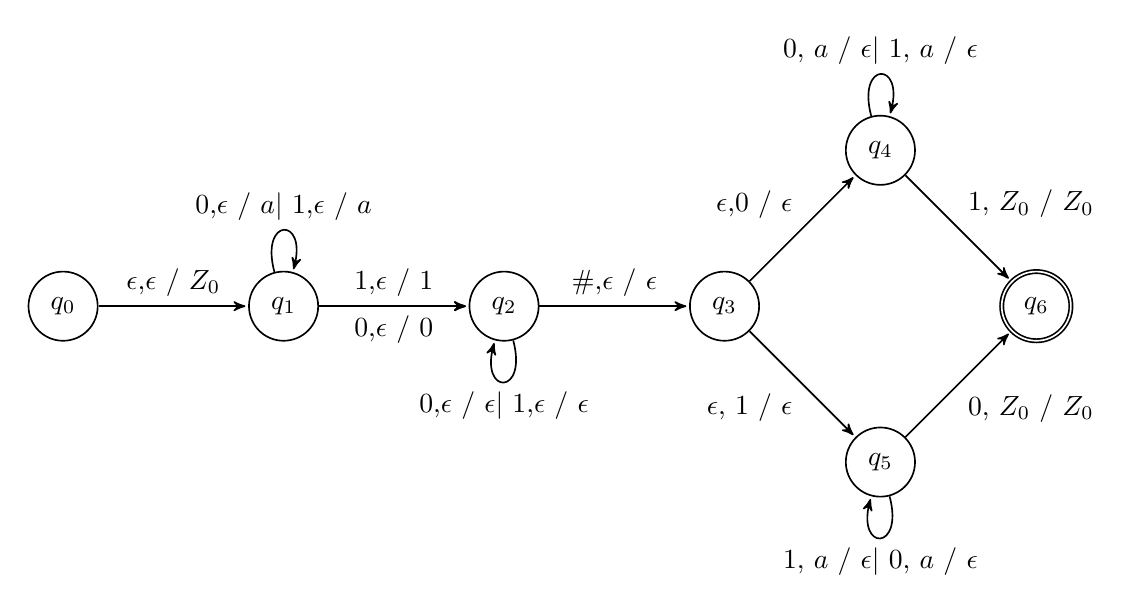
\begin{tikzpicture}[->,>=stealth',shorten >=1pt,auto,node distance=2.8cm,
                    semithick]

  \node[state] (0)              {$q_0$};
  \node[state]         (1) [right of=0] {$q_1$};
  \node[state]         (2) [right of=1] {$q_2$};
  \node[state]         (3) [right of=2] {$q_3$};
  \node[state]         (4) [above right of=3] {$q_4$};
  \node[state]         (5) [below right of=3] {$q_5$};
  \node[accepting, state]         (6) [above right of=5] {$q_6$};

  \path (0) 		edge              	    node {$\epsilon$,$\epsilon$ / $Z_0$} (1)
        (1)		edge [loop above] node {0,$\epsilon$ / $a$$|$ 1,$\epsilon$ / $a$} (1)        
        			edge              node {1,$\epsilon$ / 1} (2)
			edge [below]             node {0,$\epsilon$ / 0} (2)
        (2)edge [loop below] node {0,$\epsilon$ / $\epsilon$$|$ 1,$\epsilon$ / $\epsilon$} (2)
            edge              node {$\#$,$\epsilon$ / $\epsilon$} (3)
        (3) edge 	  		  node {$\epsilon$,0 / $\epsilon$} (4)
        	edge [below left]	  		  node {$\epsilon$, 1 / $\epsilon$} (5)
        (4) edge [loop above] node {0, $a$ / $\epsilon$$|$ 1, $a$ / $\epsilon$} (4)
            edge		 	  node {1, $Z_0$ / $Z_0$} (6)
        (5) edge [loop below] node {1, $a$ / $\epsilon$$|$ 0, $a$ / $\epsilon$} (5)
            edge [below right]node {0, $Z_0$ / $Z_0$} (6)
        
        
        
        
        ;
\end{tikzpicture}

%\section{}
%\subsection{}



\end{document}  